%!Tex Root = ../main.tex
% ./Packete.tex
% ./Design.tex
% ./Deklarationen.tex
% ./Vorbereitung.tex
% ./Aufgabe1.tex
% ./Aufgabe2.tex
% ./Aufgabe4.tex
% ./Appendix.tex

\section{Aufgabe 3}

\setcounter{exercise}{1}

\begin{frame}[allowframebreaks]{Aufgabe \thesection}{Quine-McCluskey-Algorithmus, Hypercubes und Kosten eines Polynoms}
  
        \begin{requirementsnoinc}
          \begin{itemize}
            \item $f = \bar x_1\bar x_2\bar x_3\bar x_4 + \bar x_1\bar x_2\bar x_3x_4 + \bar x_1x_2\bar x_3\bar x_4 + \bar x_1x_2\bar x_3x_4 + \bar x_1x_2x_3\bar x_4 + \bar x_1x_2x_3x_4 + x_1\bar x_2\bar x_3\bar x_4 + x_1\bar x_2x_3\bar x_4 +x_1x_2\bar x_3\bar x_4 +x_1x_2x_3\bar x_4 +x_1x_2x_3x_4$ \newline
          \end{itemize}
        \end{requirementsnoinc}
    
    \begin{solutionnoinc}
      \begin{multicols*}{2}[1. Schleifeniteration: ]
        \tiny
          $L^{\{x_1,x_2,x_3,x_4\}}_0$ \newline
          0000 \newline
          \line(1,0){20}\newline
          0001 \newline
          0100 \newline
          1000 \newline
          \line(1,0){20}\newline
          0101 \newline
          0110 \newline
          1010 \newline
          1100 \newline
          \line(1,0){20}\newline
          0111 \newline
          1110 \newline
          \line(1,0){20}\newline
          1111 \\[0.25cm]
          Prim = $\emptyset$
          \columnbreak \newline
      \end{multicols*}
    \end{solutionnoinc}
    
    \begin{solutionnoinc}
        \begin{multicols*}{2}[2. Schleifeniteration: ]
          \tiny
            $L^{\{x_1,x_2,x_3\}}_1$ \newline
            000- \newline
            \line(1,0){20}\newline
            010- \newline
            \line(1,0){20}\newline
            011- \newline
            \line(1,0){20}\newline
            111- \\[0.5cm]
            $L^{\{x_1,x_2,x_4\}}_1$ \newline
            01-0 \newline
            10-0 \newline
            \line(1,0){20}\newline
            01-1 \newline
            11-0 \newline
            \newline Prim  = $\emptyset$

            \columnbreak
            $L^{\{x_1,x_3,x_4\}}_1$ \newline
            0-00 \newline
            \line(1,0){20}\newline
            0-01 \newline
            1-00 \newline
            \line(1,0){20}\newline
            1-10 \\[0.5cm]
            $L^{\{x_2,x_3,x_4\}}_1$ \newline
            -000 \newline
            \line(1,0){20}\newline
            -100 \newline
            \line(1,0){20}\newline
            -110 \newline
            \line(1,0){20}\newline
            -111 \newline
        \end{multicols*}

    \end{solutionnoinc}

    \begin{solutionnoinc}
      \tiny
        \begin{multicols*}{2}[3. Schleifeniteration]
            $L^{\{x_1,x_2\}}_2$ \newline
            01-- \\[0.5cm]
            $L^{\{x_1,x_3\}}_2$ \newline
            0-0- \\[0.5cm]
            $L^{\{x_1,x_4\}}_2$ \newline
            1--0 \\[0.5cm]
            Prim = $\emptyset$ \newline
            \columnbreak
            \newline
            $L^{\{x_2,x_3\}}_2$ \newline
            -11- \\[0.5cm]
            $L^{\{x_2,x_4\}}_2$ \newline
            -1-0 \\[0.5cm]
            $L^{\{x_3,x_4\}}_2$ \newline
            --00 \\[0.25cm]
        \end{multicols*}
    \end{solutionnoinc}

    \begin{solution}
        \tiny
            4. Schleifeniteration\newline \newline
            $L^{\{x_1\}}_3 = \emptyset$ \newline \newline
            $L^{\{x_2\}}_3 = \emptyset$ \newline \newline
            $L^{\{x_3\}}_3 = \emptyset$ \newline \newline
            $L^{\{x_4\}}_3 = \emptyset$ \newline \newline
            Prim = \{01--, 0-0-, 1--0, -11-, -1-0, --00\} \\[0.25cm]
            $\cup_M L^M_3(f) = \emptyset \Rightarrow$ Schleifenabbruch, Prim wird zurückgegeben
    \end{solution}

    \begin{solution}
      \centering
        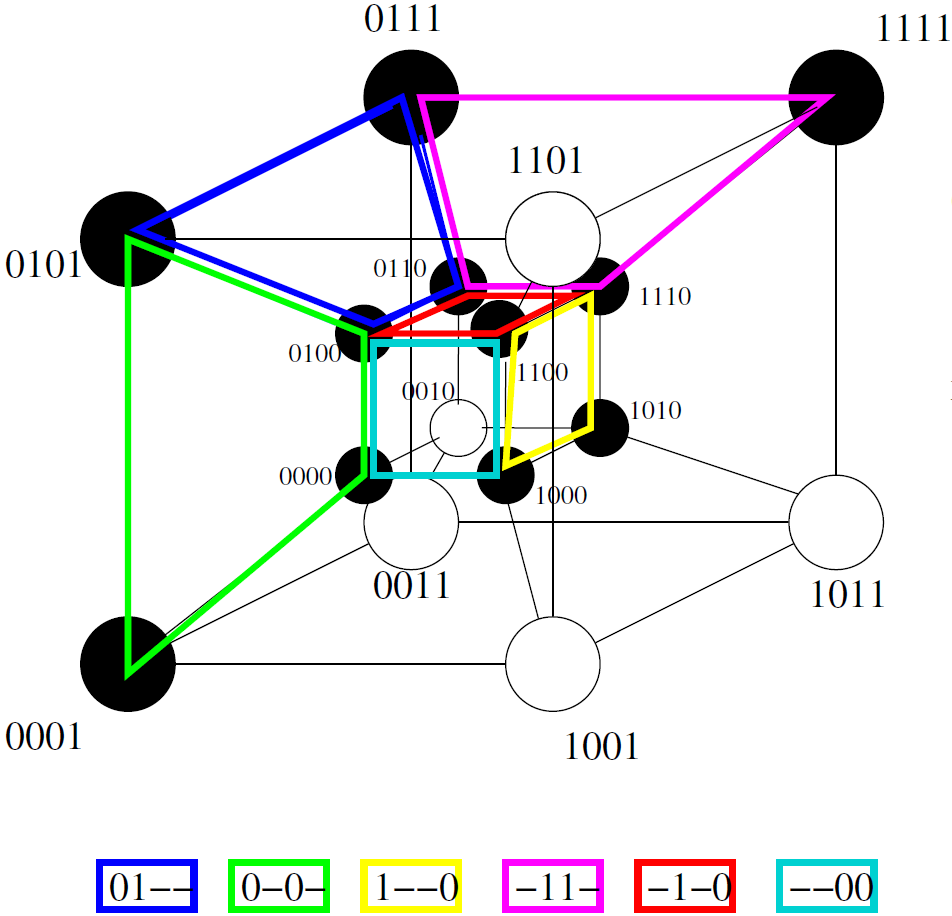
\includegraphics[height=0.6\textheight, center]{figures/HYpercube-Primimplikanten.png}
    \end{solution}

    \begin{solutionnoinc}
      \begin{itemize}
        \item \alert{primäre Kosten:} \# PLA-Zeilen, d.h. \#Monome
        \item \alert{sekundäre Kosten:} \#PLA-Transistoren, d.h. \#Literale + \#Monome
      \end{itemize}
    \end{solutionnoinc}

    \begin{solutionnoinc}
         \scriptsize $f = \bar x_1\bar x_2\bar x_3\bar x_4 + \bar x_1\bar x_2\bar x_3x_4 + \bar x_1x_2\bar x_3\bar x_4 + \bar x_1x_2\bar x_3x_4 + \bar x_1x_2x_3\bar x_4 + \bar x_1x_2x_3x_4 + x_1\bar x_2\bar x_3\bar x_4 + x_1\bar x_2x_3\bar x_4 +x_1x_2\bar x_3\bar x_4 +x_1x_2x_3\bar x_4 +x_1x_2x_3x_4$
        \begin{itemize}
          \item $cost_1$ = \#Monome = 11
          \item $cost_2$ = \#Literale + \#Monome = 44 + 11 = 55
        \end{itemize}
    \end{solutionnoinc}

    \begin{solutionnoinc}
        \scriptsize $f_{red} = \bar x_1x_2 +  \bar x_1 \bar x_3 + x_1 \bar x_4 + x_2x_3 + x_2 \bar x_4 +  \bar x_3 \bar x_4$
        \begin{itemize}
            \item $cost_1$ = \#Monome= 6
            \item $cost_2$ = \#Literale + \#Monome = 12 + 6 = 18
        \end{itemize}
    \end{solutionnoinc}
\end{frame}
